\documentclass[xetex,aspectratio=43]{beamer}
\usepackage{polyglossia}
\usepackage{fontspec}
\usepackage{xunicode} 

\usepackage{graphicx}
\graphicspath{ {../images/} }

\usepackage{listings}

\defaultfontfeatures{Ligatures=TeX}
\setmainfont{Times New Roman}
\setdefaultlanguage{russian}
\setmonofont{Courier New} 

\newfontfamily{\cyrillicfont}{Times New Roman} 
\newfontfamily{\cyrillicfontrm}{Times New Roman}
\newfontfamily{\cyrillicfonttt}{Courier New}
\newfontfamily{\cyrillicfontsf}{Arial}

% \usetheme{Pittsburgh}
\usetheme{default}
\usecolortheme{seahorse}
\setbeamersize{text margin left=7mm,text margin right=7mm} 

\beamertemplatenavigationsymbolsempty
\addtobeamertemplate{navigation symbols}{}{%
    \usebeamerfont{footline}%
    \usebeamercolor[fg]{footline}%
    \hspace{1em}%
    \insertframenumber/\inserttotalframenumber
}

\title{Выпускная квалификационная работа}
\subtitle{Система физического моделирования на основе априорного подхода обнаружения столкновений}
\author{Владислав Прекель}
\institute{ИКИТ СФУ\par КИ18-16б}
\date{Красноярск\par 20 июня 2022 г.}

\usepackage[fleqn]{mathtools}
\usepackage{unicode-math}
\usepackage{longtable}
\usepackage{hhline}

\newenvironment{Underequation}{
    \small
    \noindent
    где
    \hspace{-1.45ex}
    \setlength{\parindent}{3.5ex}
}{}

\begin{document}
\begin{frame}
    \titlepage
\end{frame}

% \begin{frame}
%     \frametitle{Модель}

%     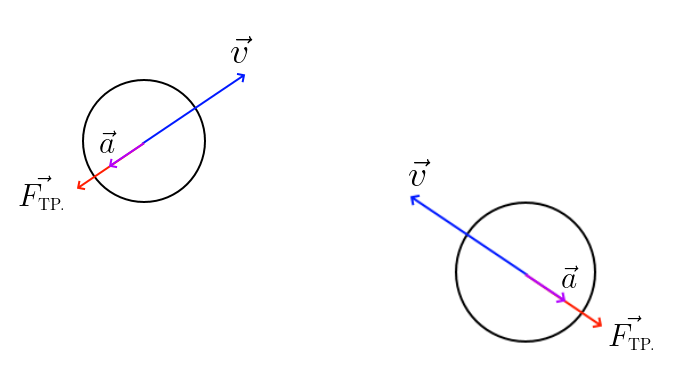
\includegraphics[height=6cm]{body_init}

% \end{frame}

% \begin{frame}
%     \frametitle{Формулы равноускоренного движения}
%     Формулы для скорости~(\ref{velocityvec_1}) и положения тела~(\ref{r_x_1}):
%     % , ускорения~(\ref{})

%     \begin{equation}\label{velocityvec_1}
%         \vec{v}(t) = \vec{v_0} + \vec{a}t
%     \end{equation}

%     \begin{equation}\label{r_x_1}
%         x(t) = x_0 + {v_0}_x t + \frac{a_x t^2}{2},
%         y(t) = y_0 + {v_0}_y t + \frac{a_y t^2}{2}
%     \end{equation}

%     % \begin{equation}
%     %     \vec{a} = \frac{\vec{F_{\text{тр.}}}}{m} = -\frac{\vec{v_0} \mu g}{\left|\vec{v_0}\right| m}
%     % \end{equation}

%     \begin{Underequation}
%         \(\vec{v}(t)\)~-- вектор скорости тела в момент времени \(t\);

%         \(\vec{v_0}\)~-- вектор начальной скорости тела;

%         \(\vec{a}\)~-- вектор ускорения тела;

%         \(x(t)\)~-- координата тела в момент времени \(t\) по оси \(X\);

%         \(x_0\)~-- координата начального положения тела по оси \(X\);

%         \(y(t)\)~-- координата тела в момент времени \(t\) по оси \(Y\);

%         \(y_0\)~-- координата начального положения тела по оси \(Y\);

%         \(a_x\)~-- проекция вектора ускорения тела \(\vec{a}\) на ось \(X\);

%         \(a_y\)~-- проекция вектора ускорения тела \(\vec{a}\) на ось \(Y\).
%     \end{Underequation}
% \end{frame}

% \begin{frame}
%     \frametitle{Тела столкнулись}

%     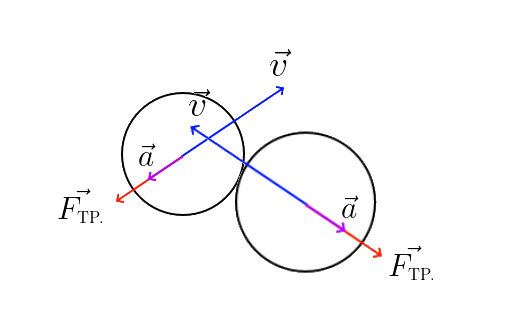
\includegraphics[height=6cm]{body_collision}

% \end{frame}

% \begin{frame}
%     \frametitle{Апостериорный подход}

%     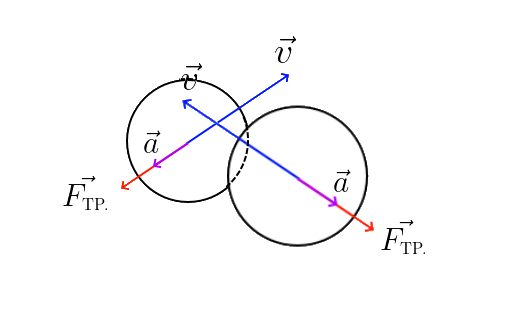
\includegraphics[height=6cm]{body_aposteriori}
% \end{frame}

\begin{frame}
    \frametitle{Априорный подход}

    Основан на том, что можно найти время столкновения через уравнение (\ref{distance_equation}):

    \begin{equation}\label{distance_equation}
        distance(t) = r_1 + r_2
    \end{equation}

    \begin{Underequation}
        \(distance(t)\)~-- расстояние между центрами двух тел в момент времени \(t\);

        \(r_1\)~-- радиус первого тела;

        \(r_2\)~-- радиус второго тела.
    \end{Underequation}

\end{frame}

\begin{frame}
    \frametitle{Цель работы}

    \textbf{Целью выпускной квалификационной работы} является
    разработка физического движка, использующего априорный подход для обнаружения столкновений.

    % для каждой задачи далее свой слайд и раздел вкр

\end{frame}

\newcommand\Constraintt{
    \frac{\left|\vec{v_0}\right|}{\left|\vec{a}\right|}
}

\newcommand\Constrainttle{
    t < \Constraintt
}

\newcommand\Constrainttge{
    t \geqslant \Constraintt
}

\begin{frame}
    \frametitle{1~Теоретические сведения}

    \begin{equation}\label{acceleration123}
        \vec{a} = -\frac{\vec{v_0}}{\left|\vec{v_0}\right|} \mu g
    \end{equation}

    \begin{equation}\label{r_x_1}
        x(t) =
        \begin{cases}
            x_0 + {v_0}_x t + \frac{a_x t^2}{2},                                                                                               & 0 \leqslant \Constrainttle, \\
            x_0 + \frac{{v_0}_x \left|\vec{v_0}\right|}{\left|\vec{a}\right|} + \frac{a_x \left|\vec{v_0}\right|^2}{2 \left|\vec{a}\right|^2}, & \Constrainttge.
        \end{cases}
    \end{equation}

    \begin{equation}\label{r_y_1}
        y(t) =
        \begin{cases}
            y_0 + {v_0}_y t + \frac{a_y t^2}{2},                                                                                               & 0 \leqslant \Constrainttle, \\
            y_0 + \frac{{v_0}_y \left|\vec{v_0}\right|}{\left|\vec{a}\right|} + \frac{a_y \left|\vec{v_0}\right|^2}{2 \left|\vec{a}\right|^2}, & \Constrainttge.
        \end{cases}
    \end{equation}

    \begin{equation}\label{bodybodyoft}
        \sqrt{(x_1(t) - x_2(t))^2 + (y_1(t) - y_2(t))^2} = r_1 + r_2
    \end{equation}

    \begin{Underequation}
        \(x(t)\),~\(y(t)\)~-- координаты положения тела в момент времени \(t\);

        \(x_0\),~\(y_0\)~-- координаты начального положения тела;

        \(\vec{v_0}\)~-- вектор начальной скорости тела;

        \(\vec{a}\)~-- вектор ускорения тела;

        \(m\)~-- масса тела;

        \(\mu\)~-- коэффициент трения тела;

        \(r\)~-- радиус тела.
    \end{Underequation}
\end{frame}

\begin{frame}
    \frametitle{2~Использованные технологии}

    \begin{itemize}
        \item OCaml~-- язык программирования;
        \item Js\_of\_ocaml~-- компилятор OCaml в JavaScript;
        \item Lwt~-- библиотека для конкурентного программирования;
        \item Core~-- стандартная библиотека;
        \item Dream~-- web-фреймворк;
        \item ppx\_inline\_test,~ppx\_expect~-- библиотеки юнит-тестирования;
        \item Sexplib~-- библиотека для сериализации и десериализации S-выражений;
        \item Bulma~-- CSS-фреймворк;
        \item Dune, opam~-- система сборки и пакетный менеджер;
        \item VS Code, OCaml Platform~-- среда разработки и плагин для работы с OCaml.
    \end{itemize}
\end{frame}

\begin{frame}
    \frametitle{3~Программная реализация}

    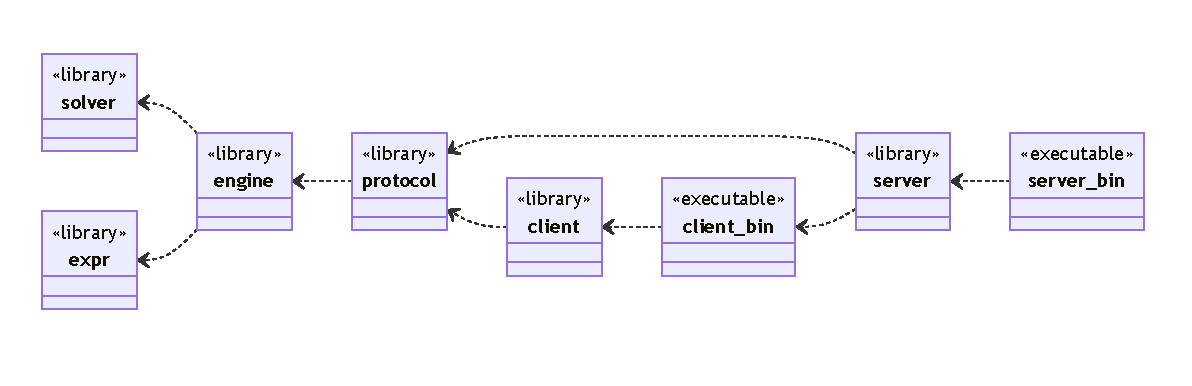
\includegraphics[width=12cm]{libsdiagram}

    \vspace{-0.6cm}
    \begin{small}
        \begin{tabular}{|p{2cm}|p{6cm}|p{1.5cm}|}
            \hline \textbf{Название подпроекта} & \textbf{Описание}                          & \textbf{Пункт и стр. ВКР} \\ \hhline{|=|=|=|}

            solver                              & Численное решение алгебраических уравнений & 3.1, с.~31                \\ \hline
            expr                                & Символьные вычисления                      & 3.2, с.~34                \\ \hline
            engine                              & Движок                                     & 3.3, с.~39                \\ \hline
            client                              & Клиентская часть приложения                & 3.4, с.~47                \\
            client\_bin                         &                                            &                           \\ \hline
            protocol                            & Общая часть приложения                     & 3.5, с.~50                \\ \cline{1-2}
            server                              & Серверная часть приложения                 &                           \\
            server\_bin                         &                                            &                           \\ \hline
        \end{tabular}
    \end{small}
\end{frame}

% \begin{frame} 
%     \frametitle{Уравнение обнаружения столкновения двух тел}

%     \begin{equation}\label{bodybodyoft}
%         \sqrt{(x_1(t) - x_2(t))^2 + (y_1(t) - y_2(t))^2} = r_1 + r_2
%     \end{equation}

%     \begin{Underequation}
%         \(x_1(t)\)~-- координата первого тела в момент времени \(t\) по оси \(X\);

%         \(x_2(t)\)~-- координата второго тела в момент времени \(t\) по оси \(X\);

%         \(y_1(t)\)~-- координата первого тела в момент времени \(t\) по оси \(Y\);

%         \(y_2(t)\)~-- координата второго тела в момент времени \(t\) по оси \(Y\);

%         \(r_1\)~-- радиус первого тела;

%         \(r_2\)~-- радиус второго тела.
%     \end{Underequation}

% \end{frame}

% \begin{frame}
%     \vspace{-1.5em}
%     \begin{align}
%         \frac{{a_x}_1^2 - {a_x}_2^2 + {a_y}_1^2 - {a_y}_2^2  }{4}                                                                    & t^4~+  \nonumber                        \\
%         + ({{v_0}_x}_1 {a_x}_1 - {{v_0}_x}_2 {a_x}_2 + {{v_0}_y}_1 {a_y}_1 - {{v_0}_y}_2 {a_y}_2)                                    & t^3~+  \nonumber                        \\
%         + ({x_0}_1 {a_x}_1 - {x_0}_2 {a_x}_2 + {y_0}_1 {a_y}_1 - {y_0}_2 {a_y}_2)                                                    & t^2~+  \nonumber                        \\
%         + 2 ({x_0}_1 {{v_0}_x}_1 - {x_0}_2 {{v_0}_x}_2 + {y_0}_1 {{v_0}_y}_1 - {y_0}_2 {{v_0}_y}_2)                                  & t~+                                     \\
%         \hspace{-1em}+ {{v_0}_x}_1^2 + {x_0}_1^2 - {{v_0}_x}_2^2 - {x_0}_2^2 + {{v_0}_y}_1^2 + {y_0}_1^2 - {{v_0}_y}_2^2 - {y_0}_2^2 & - r_1^2 - 2r_1 r_2 - r_2^2 = 0\nonumber
%     \end{align}

%     {\small
%     \begin{Underequation}
%         \({x_0}_1\)~-- начальная координата первого тела по оси \(X\);

%         \({x_0}_2\)~-- начальная координата второго тела по оси \(X\);

%         \({y_0}_1\)~-- начальная координата первого тела по оси \(Y\);

%         \({y_0}_2\)~-- начальная координата второго тела по оси \(Y\);

%         \({{v_0}_x}_1\)~-- проекция вектора начальной скорости I тела на ось \(X\);

%         \({{v_0}_y}_1\)~-- проекция вектора начальной скорости I тела на ось \(Y\);

%         \({{v_0}_x}_2\)~-- проекция вектора начальной скорости II тела на ось \(X\);

%         \({{v_0}_y}_2\)~-- проекция вектора начальной скорости II тела на ось \(Y\);

%         \({a_x}_1\)~-- проекция вектора ускорения I тела на ось \(X\);

%         \({a_y}_1\)~-- проекция вектора ускорения I тела на ось \(Y\);

%         \({a_x}_2\)~-- проекция вектора ускорения II тела на ось \(X\);

%         \({a_y}_2\)~-- проекция вектора ускорения II тела на ось \(Y\).
%     \end{Underequation}}
% \end{frame}

% \begin{frame}
%     \frametitle{Метод численного решения алгебрических уравнений}

%     \centerline{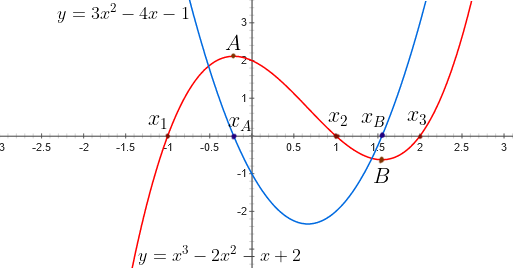
\includegraphics[height=4cm]{equation_deg3_plot}}

%     \small

%     Рассмотрим на примере уравнения \(x^3-2x^2-x+2=0\) (красное).

%     Уравнение производной \(3x^2-4x-1=0\) (синее).

%     Его корни: \(x_{A,B} = \frac{4 \pm \sqrt{28}}{6}\).

%     Тогда, корни исходного уравнения можно найти методом бисекции:

%     \(x_1\) на промежутке \((-\infty; \frac{4 - \sqrt{28}}{6}]\), будет равен \(-1\)\\
%     \(x_2\) на промежутке \([\frac{4 - \sqrt{28}}{6}; \frac{4 + \sqrt{28}}{6}]\), будет равен \(1\)\\
%     \(x_3\) на промежутке \([\frac{4 + \sqrt{28}}{6}; +\infty)\), будет равен \(2\)

% \end{frame}

% \begin{frame}
%     \frametitle{Выбор нужного корня}

%     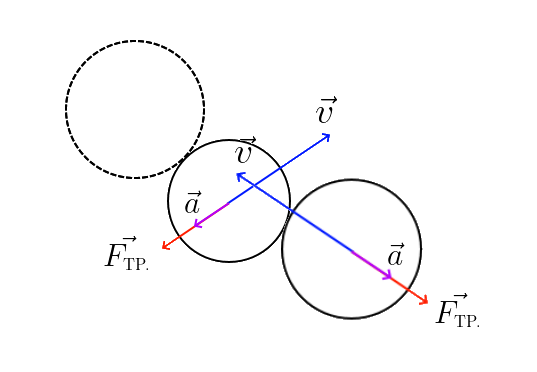
\includegraphics[height=8cm]{body_second_root}
% \end{frame}

% \begin{frame}
%     \frametitle{Уравнение обнаружения столкновения с точкой}

%     \begin{equation}\label{bodypointcollisioncoords}
%         \sqrt{(x(t) - p_x)^2 + (y(t) - p_y)^2} = r
%     \end{equation}

%     \begin{Underequation}
%         \(x(t)\)~-- координата положения тела по оси \(X\);

%         \(y(t)\)~-- координата положения тела по оси \(Y\);

%         \(r\)~-- радиус тела;

%         \(p_x\)~-- координата точки по оси \(X\);

%         \(p_y\)~-- координата точки по оси \(Y\).
%     \end{Underequation}
% \end{frame}

% \begin{frame}
%     \frametitle{Уравнение обнаружения столкновения с прямой}

%     \begin{equation}\label{bodylinecolision}
%         \frac{\left|A x(t) + B y(t) + C\right|}{\sqrt{A^2 + B^2}} = r
%     \end{equation}

%     \begin{Underequation}
%         \(A\),~\(B\),~\(C\)~-- коэффициенты общего уравнения прямой;

%         \(r\)~-- радиус тела;

%         \(x(t)\),~\(y(t)\)~-- координаты тела в момент времени \(t\).
%     \end{Underequation}

% \end{frame}

% \begin{frame}
%     \frametitle{Обработка ударов}

%     \begin{equation}\label{collisionhandle}
%         \vec{v_1^\prime} = \vec{v_1} - \frac{2 m_2}{m_1 + m_2}
%         \frac{\langle \vec{v_1} - \vec{v_2}, \vec{r_1} - \vec{r_2} \rangle }{\left| \vec{r_1} - \vec{r_2} \right|^2}
%         (\vec{r_1} - \vec{r_2})
%     \end{equation}

%     \begin{Underequation}
%         \(\langle , \rangle\)~-- скалярное произведение векторов;

%         \(\vec{v_1^\prime}\)~-- вектор скорости первого тела после удара;

%         \(\vec{v_1}\)~-- вектор скорости первого тела до удара;

%         \(\vec{v_2}\)~-- вектор скорости второго тела до удара;

%         \(\vec{r_1}\)~-- радиус-вектор положения первого тела;

%         \(\vec{r_2}\)~-- радиус-вектор положения второго тела;

%         \(m_1\)~-- масса первого тела;

%         \(m_2\)~-- масса второго тела.
%     \end{Underequation}

% \end{frame}

% \begin{frame}[fragile]
%     \frametitle{Реализация движка}

%     \footnotesize
%     \begin{lstlisting}[language=ml]
% S.Model.init ~g:1.
% |> S.Engine.recv ~action:{ time = 0.
%         ; action =
%             AddBody { id = Some id1; x0 = 350.; y0 = 200.
%                     ; r = 100.; mu = 1.; m = 10. }
%         ; until = { timespan = Some 0.; quantity = None }}
% |> S.Engine.recv ~action:{ time = 0.
%         ; action =
%             AddBody { id = Some id2; x0 = 700.; y0 = 200.
%                     ; r = 100.; mu = 1.; m = 10. }
%         ; until = { timespan = Some 0.; quantity = None }}
% |> S.Engine.recv ~action:{ time = 0.
%         ; action = GiveVelocity { id = id2; v0 = -100., 0. }
%         ; until = { timespan = None; quantity = None }}
%     \end{lstlisting}

% \end{frame}

\begin{frame}
    \frametitle{4 Интерактивная демострация возможностей}

    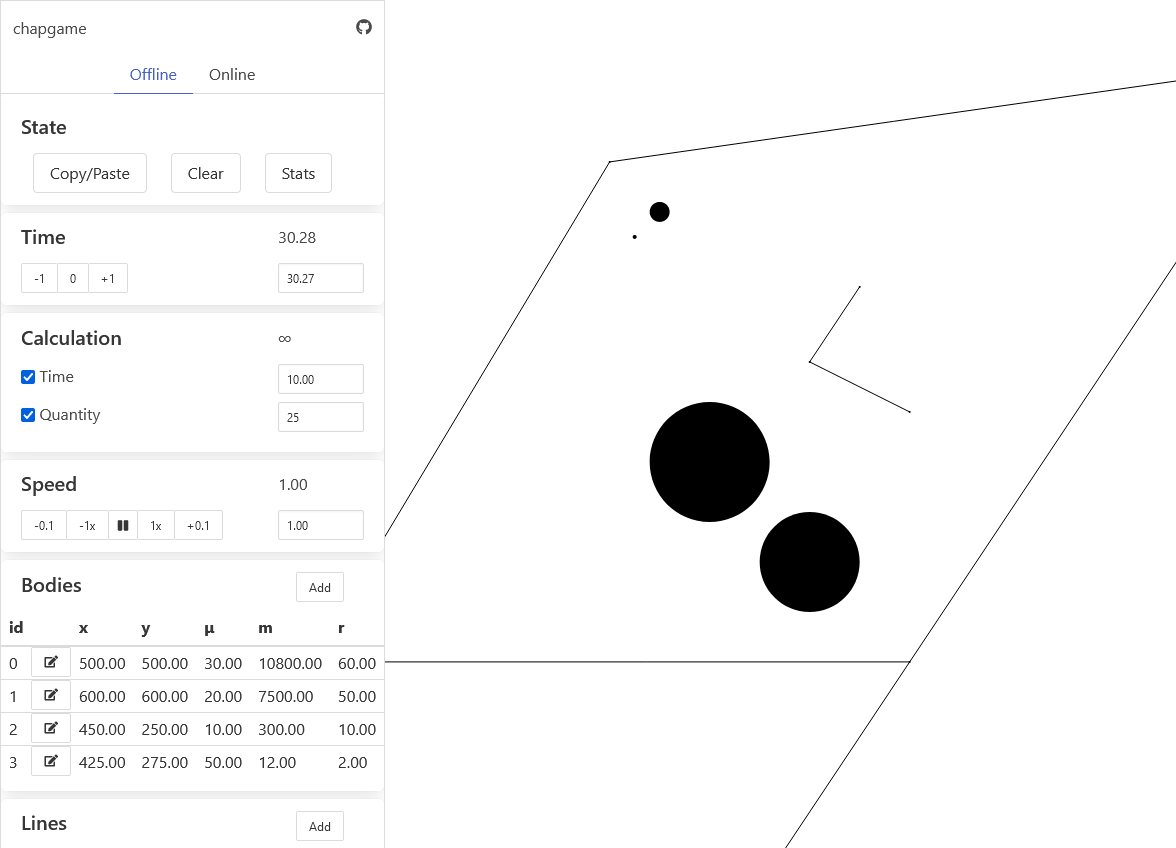
\includegraphics[height=8cm]{chapgame_1}

\end{frame}

\begin{frame}
    {\color{blue}\url{https://prekel.github.io/chapgame/}}

    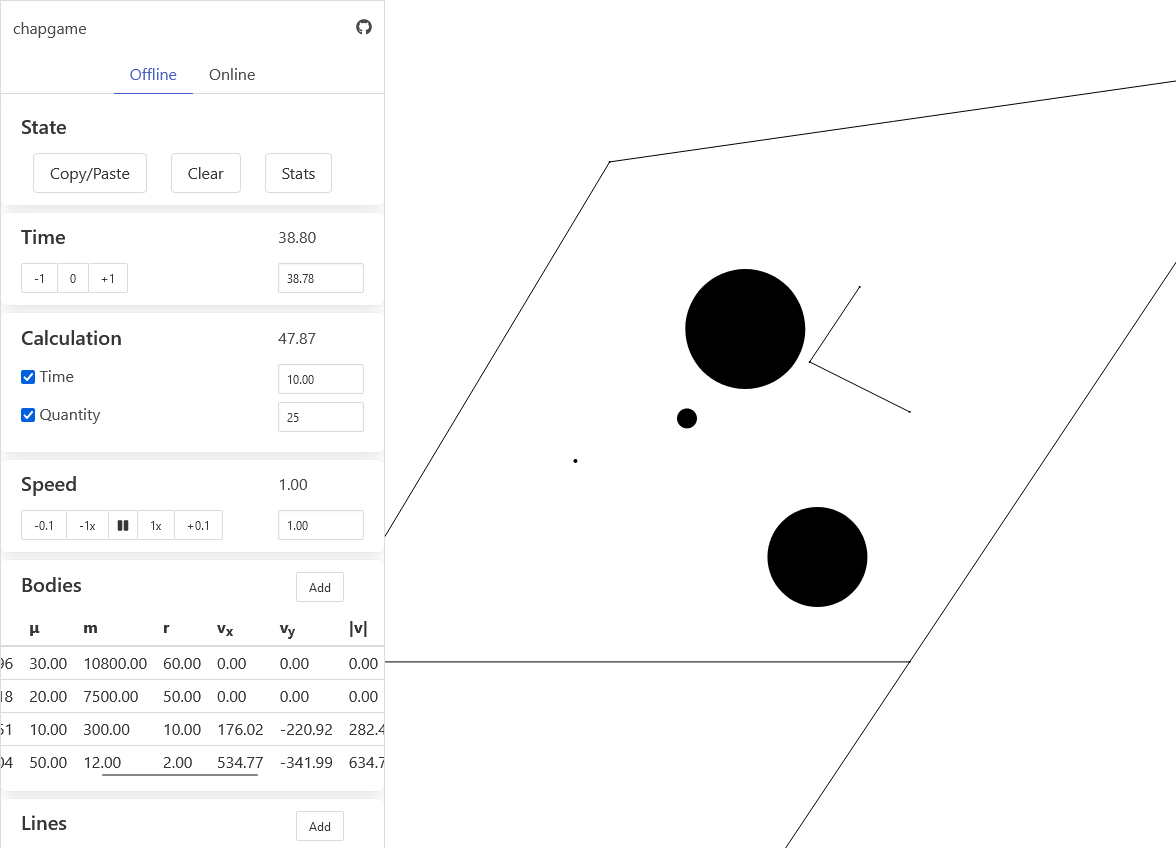
\includegraphics[height=8cm]{chapgame_2}

\end{frame}

\begin{frame}
    \frametitle{Решённые задачи}

    Были выполнены все поставленные задачи, а именно:

    \begin{itemize}
        \item в разделе~1 определена модель и систематизирована математическая база, требующаяся для реализации движка;
        \item в разделе~2 проведён обзор используемых технологий при разработке;
        \item в разделе~3 описана программная реализация физического движка и интерактивной демонстрацию его работы;
        \item в разделе~4 продемонстрирована работа движка на примерах и обозначены возможности развития.
    \end{itemize}
\end{frame}

\begin{frame}
    \titlepage
\end{frame}

\end{document}
